% TITULO
\begin{center}
    \LARGE
    \textbf{Tutorial y formato de entrega}
    \label{sec:tutorial}
    \vspace{0.4cm}
    \normalsize\\
    En la siguiente guía se mostrarán las REGLAS del informe y un tutorial de como incluir imágenes, tablas y citas. Se recomienda revisar el código para más detalles.
\end{center}

\section{TUTORIAL: Uso de la plantilla}

El archivo \verb|main.tex| va a contener algo como esto:
\begin{lstlisting}[frame=single, language=TeX]
%%%%%%%%%%%%%%%%%%%%%%%% INSTRUCCIONES Y TUTORIAL %%%%%%%%%%%%%%%%%
\begin{center}
{\LARGE\bfseries\underline{Plantilla: Informe de cierre de investigación}}
\end{center}\vspace{4ex}

La siguiente plantilla de \LaTeX{} ha sido desarrollado por la Dirección de Investigación e Innovación de la Escuela de Ingeniería UC en colaboración con \href{https://osuc.dev/}{Open Source UC} para formalizar el proceso de cierre de las actividades de Investigación de Pregrado, enmarcadas dentro del Programa IPre, y tiene los siguientes objetivos:

\begin{enumerate}
  \item Recopilar información sobre las actividades realizadas durante el curso IPre.
  \item Servir como herramienta de evaluación para el Mentor.
  \item Guiar al alumno en el proceso de comunicación científica. Para esto, el informe se ha estructurado como una publicación científica.
\end{enumerate}

A continuación, se entregan algunas direcciones generales para el uso de esta plantilla:

\begin{itemize}
  \item \textbf{Forma de entrega}: Hay que entregar dos archivos, este informe y la página de autorización \textbf{FIRMADA POR EL MENTOR}. Ambas deberán ser subidas de forma \textbf{INDEPENDIENTE} a la plataforma Gestión Ipre.
\end{itemize}

\begin{quote}
Debes ingresar a Gestión IPre, luego entrar a la pestaña de ``Investigaciones'' y hacer click en el botón ``Ver''
\end{quote}

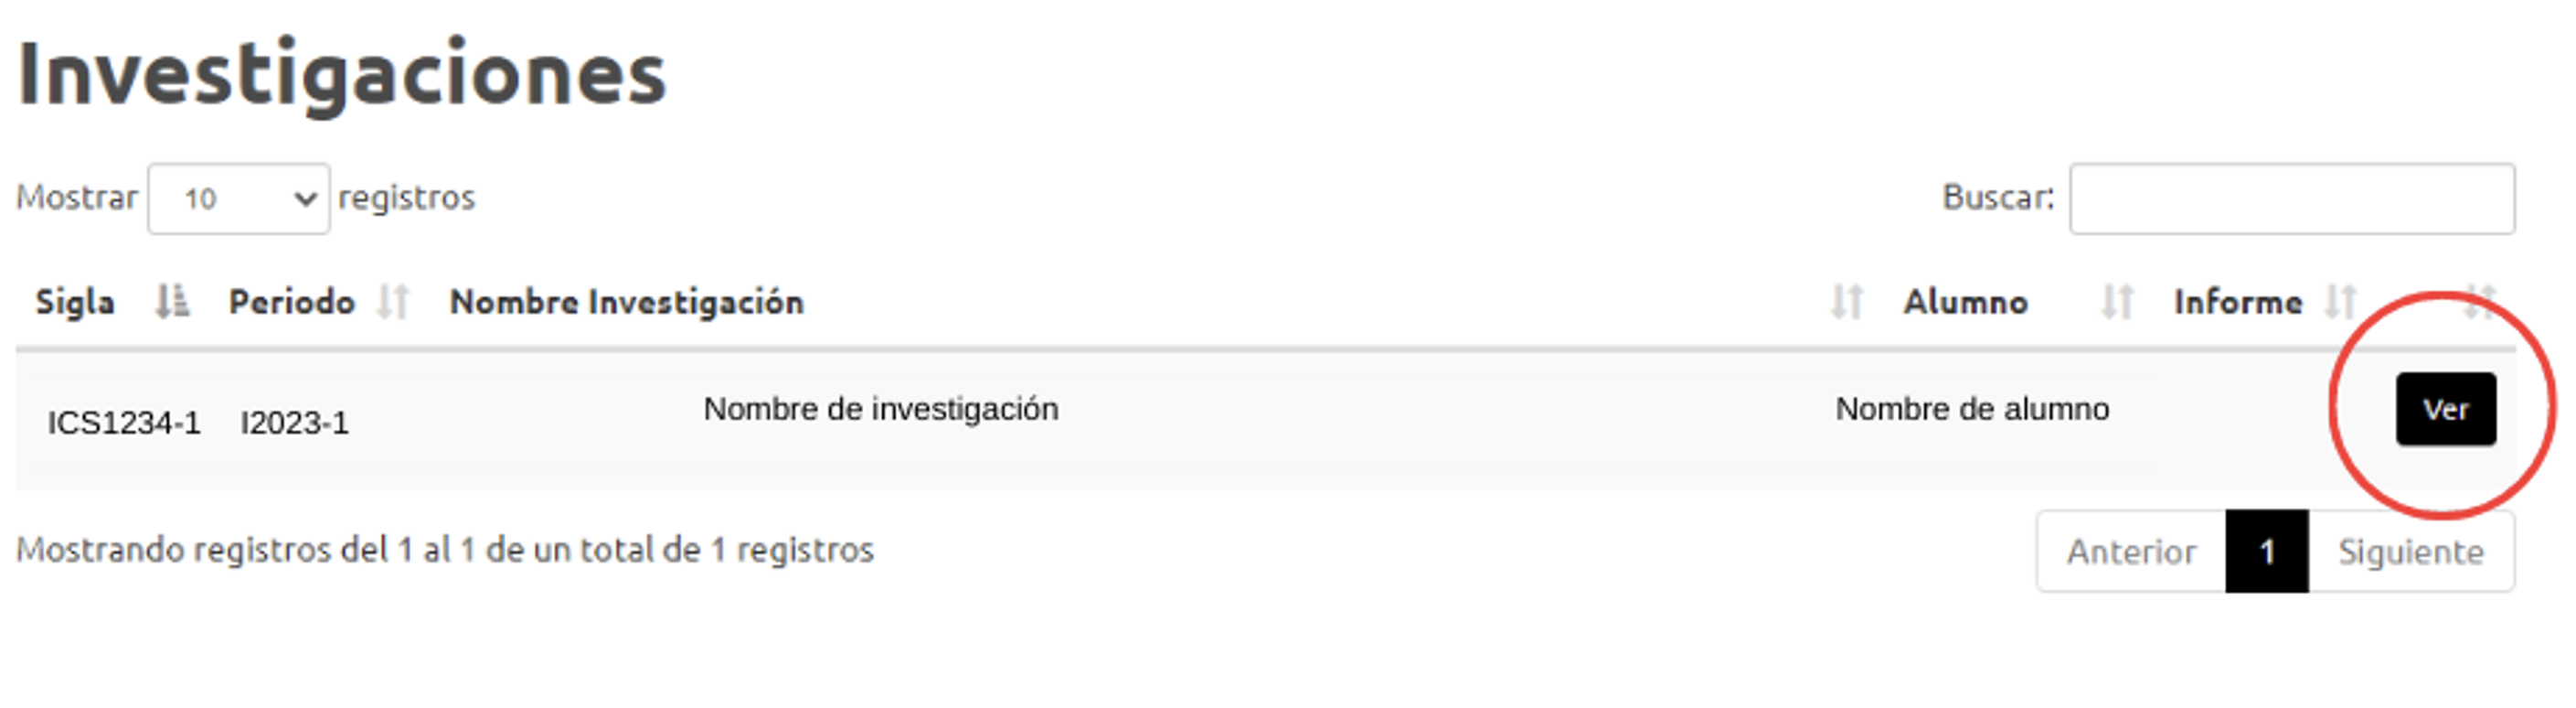
\includegraphics[width=6.13687in,height=1.85393in]{img/Imagen_1.png}

\begin{quote}
Se abrirá el detalle de la investigación, al final encontrarás el botón ``Subir Informe de Cierre'', tienes que hacer click en él para abrir el detalle del informe de cierre, en donde podrás subir el informe y la Autorización Firmada por el mentor.
\end{quote}


\begin{itemize}
  \item \underline{\textbf{Plazo de entrega}}: Dado que puedes inscribir tu Ipre durante cualquier momento del año en la plataforma Gestión Ipre, la limitante en la entrega del informe dependerá del momento en que hayas creado la investigación, obtengas un NRC e inscribas la Ipre en la plataforma Banner UC.
   Es decir, si inscribiste la IPre en Banner UC durante el periodo de inscripción de cursos para el segundo semestre, tu fecha límite de entrega del informe será al final del periodo académico del segundo semestre.\\
    Si inscribiste la IPre en Banner UC durante el periodo de inscripción de cursos para el primer semestre del siguiente año, tu fecha límite de entrega del informe será al final del periodo académico del primer semestre del siguiente año.\\
    \textbf{El no cumplimiento en la entrega del informe puede impedir la inscripción de cursos IPre en el futuro}


  \item\underline{\textbf{Extensión}}: el informe no debe contener más allá de 2.000 palabras, incluyendo resumen y cuerpo principal del artículo. Leyendas de figuras, bibliografía, autores, afiliaciones y la tabla de información incluida en este archivo no se consideran en la extensión indicada. \textbf{Informes que no respeten la extensión máxima no serán considerados}.
  \item\underline{\textbf{Figuras y tablas}}: puede incluir un máximo de 3 figuras y/o tablas para comunicar sus resultados. Las figuras y tablas deben incluir una leyenda apropiada para guiar al lector en la comprensión de sus resultados.
  \item\underline{\textbf{Estructura del escrito}}: Este informe está preparado con instrucciones para guiarlo en el uso de sus secciones de acuerdo a criterios estándar para una publicación científica. No altere la estructura indicada. Utilice las secciones y sub-secciones suministradas para facilitar la comprensión de sus resultados. \textbf{Procure usar adecuadamente el lenguaje técnico y respetar las reglas de ortografía.}
  \item\underline{\textbf{Guías para el usuario}}: este documento incluye un instructivo para el uso apropiado de referencias, preparación de material gráfico y ecuaciones. Asegúrese de seguir las instrucciones aquí entregadas. \textbf{Elimine las secciones de ayuda previo al envío del documento}.
\end{itemize}

En caso de dudas respecto de este informe, puede contactar al Coordinador del Programa de Investigación en pregrado al correo ipre@ing.puc.cl.

\newpage
 % BORRAR!
% TITULO
\begin{center}
    \LARGE
    \textbf{Tutorial y formato de entrega}
    \label{sec:tutorial}
    \vspace{0.4cm}
    \normalsize\\
    En la siguiente guía se mostrarán las REGLAS del informe y un tutorial de como incluir imágenes, tablas y citas. Se recomienda revisar el código para más detalles.
\end{center}

\section{TUTORIAL: Uso de la plantilla}

El archivo \verb|main.tex| va a contener algo como esto:
\begin{lstlisting}[frame=single, language=TeX]
%%%%%%%%%%%%%%%%%%%%%%%% INSTRUCCIONES Y TUTORIAL %%%%%%%%%%%%%%%%%
\begin{center}
{\LARGE\bfseries\underline{Plantilla: Informe de cierre de investigación}}
\end{center}\vspace{4ex}

La siguiente plantilla de \LaTeX{} ha sido desarrollado por la Dirección de Investigación e Innovación de la Escuela de Ingeniería UC en colaboración con \href{https://osuc.dev/}{Open Source UC} para formalizar el proceso de cierre de las actividades de Investigación de Pregrado, enmarcadas dentro del Programa IPre, y tiene los siguientes objetivos:

\begin{enumerate}
  \item Recopilar información sobre las actividades realizadas durante el curso IPre.
  \item Servir como herramienta de evaluación para el Mentor.
  \item Guiar al alumno en el proceso de comunicación científica. Para esto, el informe se ha estructurado como una publicación científica.
\end{enumerate}

A continuación, se entregan algunas direcciones generales para el uso de esta plantilla:

\begin{itemize}
  \item \textbf{Forma de entrega}: Hay que entregar dos archivos, este informe y la página de autorización \textbf{FIRMADA POR EL MENTOR}. Ambas deberán ser subidas de forma \textbf{INDEPENDIENTE} a la plataforma Gestión Ipre.
\end{itemize}

\begin{quote}
Debes ingresar a Gestión IPre, luego entrar a la pestaña de ``Investigaciones'' y hacer click en el botón ``Ver''
\end{quote}

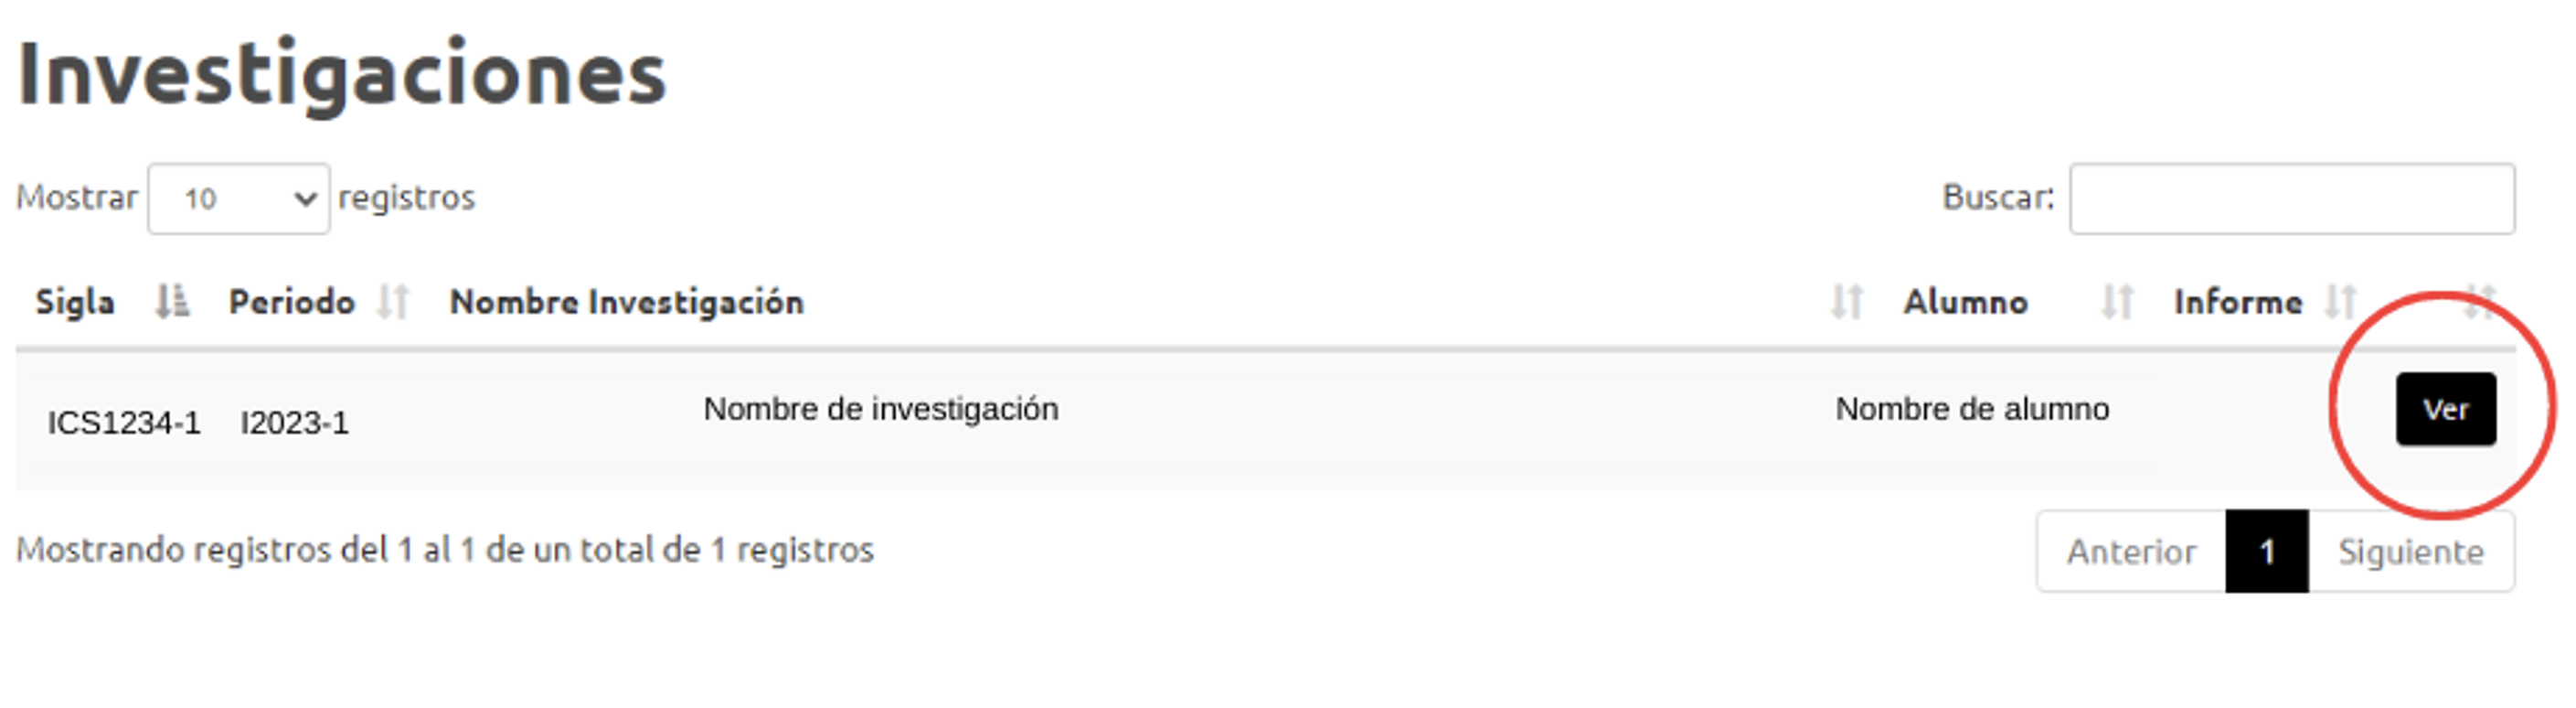
\includegraphics[width=6.13687in,height=1.85393in]{img/Imagen_1.png}

\begin{quote}
Se abrirá el detalle de la investigación, al final encontrarás el botón ``Subir Informe de Cierre'', tienes que hacer click en él para abrir el detalle del informe de cierre, en donde podrás subir el informe y la Autorización Firmada por el mentor.
\end{quote}


\begin{itemize}
  \item \underline{\textbf{Plazo de entrega}}: Dado que puedes inscribir tu Ipre durante cualquier momento del año en la plataforma Gestión Ipre, la limitante en la entrega del informe dependerá del momento en que hayas creado la investigación, obtengas un NRC e inscribas la Ipre en la plataforma Banner UC.
   Es decir, si inscribiste la IPre en Banner UC durante el periodo de inscripción de cursos para el segundo semestre, tu fecha límite de entrega del informe será al final del periodo académico del segundo semestre.\\
    Si inscribiste la IPre en Banner UC durante el periodo de inscripción de cursos para el primer semestre del siguiente año, tu fecha límite de entrega del informe será al final del periodo académico del primer semestre del siguiente año.\\
    \textbf{El no cumplimiento en la entrega del informe puede impedir la inscripción de cursos IPre en el futuro}


  \item\underline{\textbf{Extensión}}: el informe no debe contener más allá de 2.000 palabras, incluyendo resumen y cuerpo principal del artículo. Leyendas de figuras, bibliografía, autores, afiliaciones y la tabla de información incluida en este archivo no se consideran en la extensión indicada. \textbf{Informes que no respeten la extensión máxima no serán considerados}.
  \item\underline{\textbf{Figuras y tablas}}: puede incluir un máximo de 3 figuras y/o tablas para comunicar sus resultados. Las figuras y tablas deben incluir una leyenda apropiada para guiar al lector en la comprensión de sus resultados.
  \item\underline{\textbf{Estructura del escrito}}: Este informe está preparado con instrucciones para guiarlo en el uso de sus secciones de acuerdo a criterios estándar para una publicación científica. No altere la estructura indicada. Utilice las secciones y sub-secciones suministradas para facilitar la comprensión de sus resultados. \textbf{Procure usar adecuadamente el lenguaje técnico y respetar las reglas de ortografía.}
  \item\underline{\textbf{Guías para el usuario}}: este documento incluye un instructivo para el uso apropiado de referencias, preparación de material gráfico y ecuaciones. Asegúrese de seguir las instrucciones aquí entregadas. \textbf{Elimine las secciones de ayuda previo al envío del documento}.
\end{itemize}

En caso de dudas respecto de este informe, puede contactar al Coordinador del Programa de Investigación en pregrado al correo ipre@ing.puc.cl.

\newpage
 % BORRAR!
% TITULO
\begin{center}
    \LARGE
    \textbf{Tutorial y formato de entrega}
    \label{sec:tutorial}
    \vspace{0.4cm}
    \normalsize\\
    En la siguiente guía se mostrarán las REGLAS del informe y un tutorial de como incluir imágenes, tablas y citas. Se recomienda revisar el código para más detalles.
\end{center}

\section{TUTORIAL: Uso de la plantilla}

El archivo \verb|main.tex| va a contener algo como esto:
\begin{lstlisting}[frame=single, language=TeX]
%%%%%%%%%%%%%%%%%%%%%%%% INSTRUCCIONES Y TUTORIAL %%%%%%%%%%%%%%%%%
\begin{center}
{\LARGE\bfseries\underline{Plantilla: Informe de cierre de investigación}}
\end{center}\vspace{4ex}

La siguiente plantilla de \LaTeX{} ha sido desarrollado por la Dirección de Investigación e Innovación de la Escuela de Ingeniería UC en colaboración con \href{https://osuc.dev/}{Open Source UC} para formalizar el proceso de cierre de las actividades de Investigación de Pregrado, enmarcadas dentro del Programa IPre, y tiene los siguientes objetivos:

\begin{enumerate}
  \item Recopilar información sobre las actividades realizadas durante el curso IPre.
  \item Servir como herramienta de evaluación para el Mentor.
  \item Guiar al alumno en el proceso de comunicación científica. Para esto, el informe se ha estructurado como una publicación científica.
\end{enumerate}

A continuación, se entregan algunas direcciones generales para el uso de esta plantilla:

\begin{itemize}
  \item \textbf{Forma de entrega}: Hay que entregar dos archivos, este informe y la página de autorización \textbf{FIRMADA POR EL MENTOR}. Ambas deberán ser subidas de forma \textbf{INDEPENDIENTE} a la plataforma Gestión Ipre.
\end{itemize}

\begin{quote}
Debes ingresar a Gestión IPre, luego entrar a la pestaña de ``Investigaciones'' y hacer click en el botón ``Ver''
\end{quote}

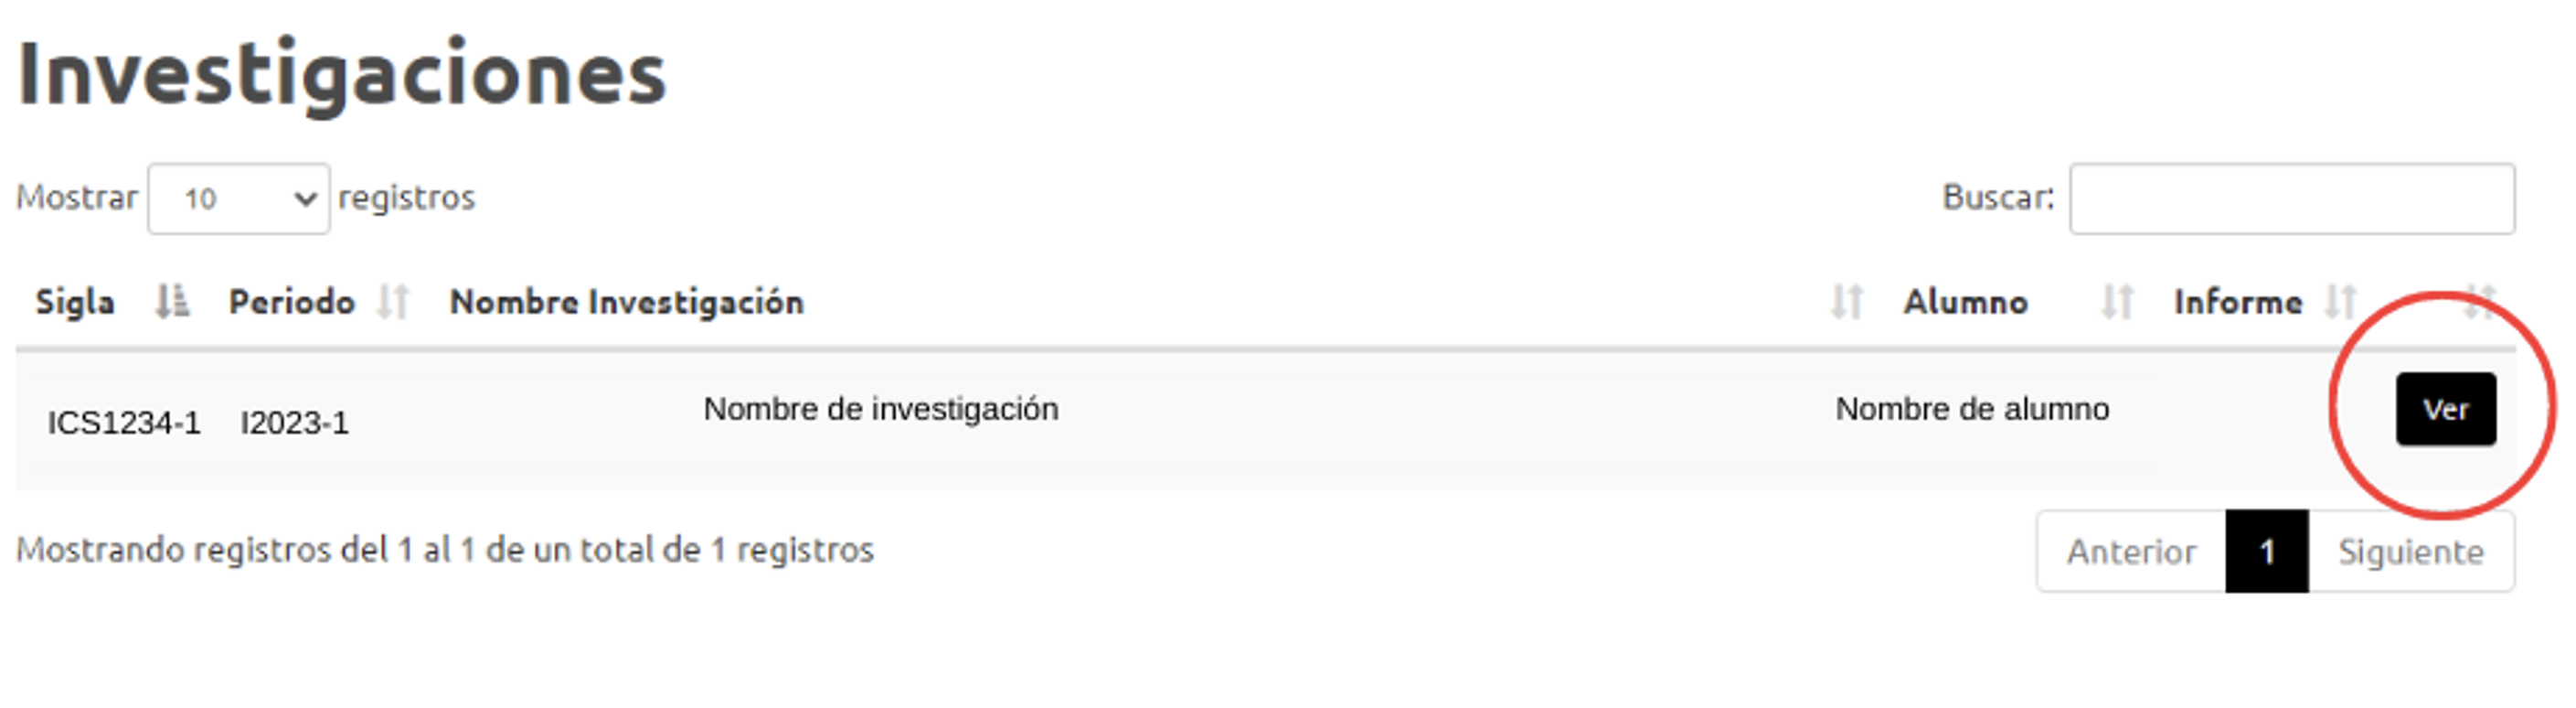
\includegraphics[width=6.13687in,height=1.85393in]{img/Imagen_1.png}

\begin{quote}
Se abrirá el detalle de la investigación, al final encontrarás el botón ``Subir Informe de Cierre'', tienes que hacer click en él para abrir el detalle del informe de cierre, en donde podrás subir el informe y la Autorización Firmada por el mentor.
\end{quote}


\begin{itemize}
  \item \underline{\textbf{Plazo de entrega}}: Dado que puedes inscribir tu Ipre durante cualquier momento del año en la plataforma Gestión Ipre, la limitante en la entrega del informe dependerá del momento en que hayas creado la investigación, obtengas un NRC e inscribas la Ipre en la plataforma Banner UC.
   Es decir, si inscribiste la IPre en Banner UC durante el periodo de inscripción de cursos para el segundo semestre, tu fecha límite de entrega del informe será al final del periodo académico del segundo semestre.\\
    Si inscribiste la IPre en Banner UC durante el periodo de inscripción de cursos para el primer semestre del siguiente año, tu fecha límite de entrega del informe será al final del periodo académico del primer semestre del siguiente año.\\
    \textbf{El no cumplimiento en la entrega del informe puede impedir la inscripción de cursos IPre en el futuro}


  \item\underline{\textbf{Extensión}}: el informe no debe contener más allá de 2.000 palabras, incluyendo resumen y cuerpo principal del artículo. Leyendas de figuras, bibliografía, autores, afiliaciones y la tabla de información incluida en este archivo no se consideran en la extensión indicada. \textbf{Informes que no respeten la extensión máxima no serán considerados}.
  \item\underline{\textbf{Figuras y tablas}}: puede incluir un máximo de 3 figuras y/o tablas para comunicar sus resultados. Las figuras y tablas deben incluir una leyenda apropiada para guiar al lector en la comprensión de sus resultados.
  \item\underline{\textbf{Estructura del escrito}}: Este informe está preparado con instrucciones para guiarlo en el uso de sus secciones de acuerdo a criterios estándar para una publicación científica. No altere la estructura indicada. Utilice las secciones y sub-secciones suministradas para facilitar la comprensión de sus resultados. \textbf{Procure usar adecuadamente el lenguaje técnico y respetar las reglas de ortografía.}
  \item\underline{\textbf{Guías para el usuario}}: este documento incluye un instructivo para el uso apropiado de referencias, preparación de material gráfico y ecuaciones. Asegúrese de seguir las instrucciones aquí entregadas. \textbf{Elimine las secciones de ayuda previo al envío del documento}.
\end{itemize}

En caso de dudas respecto de este informe, puede contactar al Coordinador del Programa de Investigación en pregrado al correo ipre@ing.puc.cl.

\newpage
 % BORRAR!
% TITULO
\begin{center}
    \LARGE
    \textbf{Tutorial y formato de entrega}
    \label{sec:tutorial}
    \vspace{0.4cm}
    \normalsize\\
    En la siguiente guía se mostrarán las REGLAS del informe y un tutorial de como incluir imágenes, tablas y citas. Se recomienda revisar el código para más detalles.
\end{center}

\section{TUTORIAL: Uso de la plantilla}

El archivo \verb|main.tex| va a contener algo como esto:
\begin{lstlisting}[frame=single, language=TeX]
%%%%%%%%%%%%%%%%%%%%%%%% INSTRUCCIONES Y TUTORIAL %%%%%%%%%%%%%%%%%
\input{content/instrucciones} % BORRAR!
\input{content/minitutorial}  % BORRAR!
%%%%%%%%%%%%%%%%%%%%%%%% CONTENIDO %%%%%%%%%%%%%%%%%%%%%%%%%%%%%%%%
% Seleccionar uno de los siguientes apartados:
\input{content/investigacion_experimental}
\input{content/informe_bibliografico}
%%%%%%%%%%%%%%%%%%%%%%% FICHA DE INFORMACION %%%%%%%%%%%%%%%%%%%%%%
\fichaparteuno{Nombre completo}{Nombre mentor}
        {ejemplo@uc.cl}{ejemplo@uc.cl}
        {Sigla curso}{Seccion}
        {Año}{Semestre}
        {Titulo investigación}
\fichapartedos{Titulo del proyecto}
        {Fecha inicio}{\today}
        {}{X} % Escoger una
        {X}{} % Escoger una
        {NOMBRE MENTOR PRINCIPAL}{\today}

\end{lstlisting}

Por lo tanto, es importante considerar las siguientes indicaciones:
\begin{itemize}
    \item Al entregar el informe, se debe \textbf{eliminar} la sección de instrucciones y tutorial.
    \item En la parte de contenido, se debe seleccionar \textbf{únicamente 1} de los dos apartados disponibles.
    \item Se debe completar e imprimir la "Ficha de información" para que sea firmada y luego entregada en formato digital. \textbf{No} se tiene que incluir en el informe final. Una vez que esté firmada y en formato impreso, se debe eliminar dicha sección.
\end{itemize}


\section{TUTORIAL: Imágenes}

El contenido de la figura deberá estar en idioma inglés. La resolución de las imágenes debe ser de al menos 300 dpi y cada figura debe caber en una página tamaño carta (8,5 x 11 pulgadas). La revista utiliza tres tamaños estándar de figura: 1 columna, 85 mm; 1,5 columnas, 114 mm; y 2 columnas, 174 mm (ancho total de la página). Por favor, considere estas dimensiones al crear sus ilustraciones, aunque estas podrán ser encogidas durante el proceso de diseño editorial.

Los textos de las figuras deben ser en mayúsculas solo para la primera palabra de cada frase. Las unidades de medida deben tener un espacio entre el número y la unidad y seguir la nomenclatura internacional SI (por ejemplo, h en vez de hrs.). La numeración debe incluir “,” para separación de miles y “.” para separación de decimales.


\subsection{Imagen centrada}
En esta plantilla hay 2 formas de incluir imágenes. La primera es la más compleja y manual que aparece en el código comentado.
%\begin{figure}[H]
%    \centering
%    \begin{measuredfigure} % Lo usamos para aliniar el caption
%        
\includegraphics[width=0.2\textwidth]{img/cuadradoejemplo.png} % Alternativa \includegraphics[height=3cm]{}
%        \caption{Título de la imagen}
%        \label{img:label_referencia0}
%    \end{measuredfigure}
%\end{figure}

La segunda forma de incluir imágenes es la más sencilla, solo se tiene que usar el comando personalizado:
\begin{verbatim}
\fig[label]{Titulo}{tamaño}{ruta_imagen}
Ejemplo:
\fig[referencia1]{Titulo de la imagen 1}{width = 0.2\textwidth}{img/cuadradoejemplo.png}
\end{verbatim}

\fig[labelreferencia1]{Titulo de la imagen 1}{width = 0.2\textwidth}{img/cuadradoejemplo.png}


\subsection{Imágenes compuestas}

Para crear imágenes compuestas se requiere una mayor personalización, por lo que no se incluyo un comando para simplificarlo. Se pueden fijar en el código de este apartado.

\begin{figure}[H]
 \centering
  \subfloat[Foto1]{
    
\includegraphics[width=0.2\textwidth]{cuadradoejemplo.png}}
    \label{f:label_foto1}
  \subfloat[Foto2]{
    
\includegraphics[width=0.2\textwidth]{cuadradoejemplo.png}}
    \label{f:label_foto2}
  \subfloat[Foto3]{
    
\includegraphics[width=0.2\textwidth]{cuadradoejemplo.png}}
    \label{f:label_foto3}
 \caption{Múltiples imágenes}
 \label{f:label_multiples_imagenes}
\end{figure}

\subsection{Imágenes alineadas}
Si se desea incluir una imagen a la izquierda o derecha de un párrafo, se puede usar el siguiente comando (Poniendo \{r\} o \{l\} dependiendo del caso):
\begin{verbatim}
\figposition[label]{Titulo}{tamaño}{ruta_imagen}{posicion_r/l}
Ejemplo:
\figposition[referencia2]{Imagen referencia }{height=3cm}{img/cuadradoejemplo.png}{r}
\end{verbatim}

\figposition[referencia2]{Imagen referencia }{height=3cm}{img/cuadradoejemplo.png}{r}
% FORMA MANUAL:
%\begin{wrapfigure}{r}{0.25\textwidth} % Margen del texto
%    \centering
%    \begin{measuredfigure}
%        \caption{Imagen referencia 2}
%        
\includegraphics[height=3cm]{img/cuadradoejemplo.png} %[scale=0.1]
%        \label{img:referencia2}
%    \end{measuredfigure}
%\end{wrapfigure}
\textcolor{silver}{
    Lorem Ipsum is simply dummy text of the printing and typesetting industry. Lorem Ipsum has been the industry's standard dummy text ever since the 1500s, when an unknown printer took a galley of type and scrambled it to make a type specimen book. It has survived not only five centuries, but also the leap into electronic typesetting, remaining essentially unchanged.
    }

%%%%%%%%%%%%%%%%%%%%%%%%%%%%%%%%%%%%%%%%%%%%%%%%%%%%%%%
\newpage
\section{TUTORIAL: Tablas}

Se requiere utilizar "," para la unidad decimal, tanto en las tablas como en el texto.

Hacer tablas en \LaTeX es muy engorroso, por lo que presentamos 3 alternativas. Sin embargo, es necesario aclarar que para que se respete el formato de las tablas, \textbf{se tiene que poner el catión SOBRE la tabla.}

\subsection{Generador online}
Hay muchas páginas para generar tablas automáticamente, una alternativa es \href{https://www.tablesgenerator.com}{tablesgenerator}, sin embargo, este método genera muchas líneas innecesarias y cuando se incorporan párrafos muy grandes hay que ajustar las palabras.

\subsection{Insertar una imagen como tabla}
Se puede incorporar una imagen (De Excel, por ejemplo) como si fuera una tabla. El único inconveniente es que no va a permitir seleccionar el texto en el pdf generado. Al igual que con las imágenes, hay un comando personalizado y un código manual comentado.
\begin{verbatim}
\tableimage[label]{Titulo}{tamaño}{ruta_imagen}
Ejemplo:
\tableimage[referencia3]{Tabla de referencia 1}{height=3cm}{img/tablaejemplo.png}
\end{verbatim}



\tableimage[referencia3]{Titulo de la tabla de referencia}{height=3cm}{img/tablaejemplo.png}

% Tabla manual:
%\begin{table}[H]
%    \centering
%    \begin{measuredfigure}
%        \caption{Tabla de referencia 1}
%        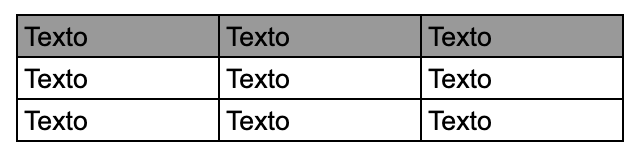
\includegraphics[height=3cm]{img/tablaejemplo.png}
%        \label{img:referencia3}
%    \end{measuredfigure}
%    \\ \textit{\scriptsize{Texto opcional al el pie de Tabla.}}
%\end{table}

\newpage
\subsection{Usar plantillas}
Pueden copiar y modificar el código que aparece a continuación en él .tex:

\begin{minipage}[H]{0.49\textwidth}
    \begin{table}[H]
        \centering
        \begin{measuredfigure}
            \caption{Tabla de referencia 2}
            \begin{tabular}{| l | c | r |}
            \hline
                \textbf{Texto} & \textbf{Texto} & \textbf{Texto} \\ \hline
                Textoblabla    & Textoblabla   & Textoblabla \\ \hline
                Texto    & Texto   & Texto \\ \hline
            \end{tabular}
        \end{measuredfigure}
    \end{table}
\end{minipage}
\begin{minipage}[H]{0.49\textwidth}
    \begin{table}[H]
        \centering
        \begin{measuredfigure}
            \caption{Tabla de referencia 3}
            \begin{tabular}{l l l}
            \toprule
                \textbf{Texto} & \textbf{Texto} & \textbf{Texto} \\
                \midrule
                Textoblabla    & Textoblabla   & Textoblabla \\
                Texto    & Texto   & Texto \\
                \bottomrule
            \end{tabular}
        \end{measuredfigure}
    \end{table}
\end{minipage}

\section{Fórmulas y Ecuaciones}

En LaTeX, puedes incluir fórmulas y ecuaciones matemáticas dentro del texto o en línea, como $E = mc^2$, utilizando el símbolo del dólar (\$) para abrir y cerrar la fórmula. Pueden buscar guías detalladas sobre como funcionan, sin embargo, con el correo universitario los estudiantes tienen acceso a \href{https://mathpix.com}{Mathpix} una aplicación móvil y de escritorio que digitaliza fórmulas en el formato deseado con muy buenos resultados.

También puedes crear ecuaciones numeradas como esta:

\begin{equation}
    a^2 + b^2 = c^2
\end{equation}

Puedes alinear varias ecuaciones utilizando el entorno \verb|\begin{align}|:

\begin{align}
    x &= 2y + 3 \\
    3x - 5y &= 9
\end{align}

Si no quieres numerar una ecuación, utiliza el entorno \verb|\begin{align*}|:

\begin{align*}
    f(x) &= x^2 + 2x + 1 \\
    &= (x + 1)^2
\end{align*}

%%%%%%%%%%%%%%%%%%%%%%%%%%%%%%%%%%%%%%%%%%%%%%%%%%%%%%%
\newpage
\section{TUTORIAL: Citación}

Tal como se indica en el archivo main, existen dos enfoques para agregar bibliografía en un documento \LaTeX. El primero implica la utilización de un archivo .bib, lo cual automatiza el proceso de citación. Al emplear esta técnica, se debe incluir el estilo de bibliografía mediante el comando \verb|\bibliographystyle{apacite}|, y luego referirse al archivo .bib con la instrucción \verb|\bibliography{mybib.bib}|, donde mybib.bib es el nombre del archivo de bibliografía. Este método es altamente automatizado y simplifica la tarea de referenciar.

La segunda opción implica agregar la bibliografía directamente en un archivo \textbf{.tex}, lo que resulta más manual. En este caso, se citan las fuentes manualmente utilizando comandos como \verb|\cite{key}| y se define el formato de la bibliografía utilizando \verb|\begin{thebibliography}{99}| y \verb|\end{thebibliography}|. Aunque menos automatizado que el primer enfoque, esta opción permite un mayor control sobre la presentación y organización de las referencias en el documento.

\subsection{Citas extensas}

Para citación extensa en formato APA, citas con más de 40 palabras, se sugiere el uso del siguiente comando personalizado:

\begin{verbatim}
    \quotex{cita}
    Ejemplo:
    \quotex{\lipsum (Autor, Año)}
\end{verbatim}

\quotex{...texto extenso... (Autor, Año)}

Puedes realizarlo de forma manual modificando el código comentado

%Cita extensa APA manual:

%\begin{flushright}
%    \begin{minipage}{0.96\linewidth}
%        \vspace{5pt}
%        {\small
%            %Acá va la cita
%        }
%        \vspace{5pt}
%    \end{minipage}
%\end{flushright}

\newpage  % BORRAR!
%%%%%%%%%%%%%%%%%%%%%%%% CONTENIDO %%%%%%%%%%%%%%%%%%%%%%%%%%%%%%%%
% Seleccionar uno de los siguientes apartados:
% TITULO
\begin{center}
    \LARGE
    \textbf{Título de la investigación experimental}
    \label{sec:investigacion_experimental}
    
    \vspace{0.4cm}
    \large
    Alumno $1^a$, (…) Profesor $1^b$ 

    \vspace{0.4cm}
\end{center}

% Informacion
\begin{enumerate}[label=\alph*]
    \item Indicar major o departamento, indicar escuela o
facultad, indicar universidad. Año de carrera, e-mail
    \item Indicar departamento, indicar escuela o facultad,
indicar universidad. Incluir categoría profesor, e-mail
\end{enumerate}

\hrulefill

\section*{Resumen}

El resumen debe indicar brevemente cuál es el problema, el objetivo o
hipótesis del estudio, métodos utilizados, resultados y conclusiones.
Además, debe ser independiente del texto principal, es decir, debe
entenderse por sí solo. \textbf{Extensión máxima: 300 palabras.}

\emph{\textbf{Palabras clave:}} incluir hasta 5 palabras claves que se
relacionen con el alcance y objetivo de la investigación.

\hrulefill

\textbf{NOTA: Si usted realizó una investigación de tipo
bibliográfica (recopilando información sin datos experimentales), ignore
esta plantilla y continúe \hyperref[sec:investigacion_bibliografica]{aquí}. De lo contrario, elimine esta instrucción.}

\section{Introducción}

Escriba aquí una breve introducción al tema de investigación, incluyendo
el estado del arte, su contingencia en Chile y/o en el mundo y el
desafío particular a resolver. La introducción debe: (1) indicar el
problema que justifica la investigación y/o la hipótesis en la que ésta
se basa, (2) los antecedentes o resultados de otros artículos que serán
utilizados durante el artículo, y (3) una explicación del enfoque
general y los objetivos del trabajo.

\subsection{Subsecciones}

Si necesita utilizar subsecciones para estructurar su escrito, puede
realizarlo siguiendo este formato. Esto es válido para las secciones
principales de este documento (Introducción, Metodología, Resultados y
Conclusión).

\section{Experimentación o metodología (según corresponda)}

En esta sección se describirá brevemente la metodología relevante en
relación al trabajo, indicando los experimentos o simulaciones
realizadas. De ser adecuado, incluya una descripción de los materiales
utilizados. La sección de metodología debe ser ordenada de manera lógica
(cronológicamente, por experimento, etc.) y puede incluir figuras,
tablas y/o referencias.

Algunas sugerencias de subsecciones son: Instrumentos, Grupos de estudio

\section{Resultados y discusión}

Describa y explique los principales resultados del trabajo presentado,
incluyendo un contraste con el estado del arte. Use tablas y figuras que
ayuden a una mejor comprensión de los resultados encontrados. Le
recordamos que la discusión debe incluir una interpretación de los
resultados obtenidos a la luz del problema o hipótesis planteados en la
introducción.

\section{Conclusiones}

Describa aquí las conclusiones del trabajo presentado. En ellas se deben
mencionar los resultados obtenidos más relevantes, las inferencias que
se extraen a partir de los resultados y las implicancias para el uso
práctico de ellas. Es importante destacar si
la hipótesis presentada fue refutada o no y cuál es el aporte de los
resultados al problema planteado.

\section*{Agradecimientos}

Puede incluir un reconocimiento a las personas o entidades que hayan
contribuido al estudio. Se debe especificar el tipo de apoyo entregado.

\section{Glosario}\label{glosario}

Debe incluir un máximo de 10 palabras o conceptos para
facilitar la lectura del público no especialista. La palabra a definir
debe aparecer en \textbf{NEGRITA} y mayúsculas la primera vez que se mencione en
el texto. Las palabras clave deben ser incluidas en el glosario y estar
listadas en orden alfabético. Evite anglicismos a menos que sea
estrictamente necesario.\\ Utilice el siguiente formato:


\begin{description}
    \definiritem{Palabra 1}{Definición de la palabra 1.}
    \definiritem{Palabra 2}{Definición de la palabra 2.}
    \definiritem{Palabra 3}{Definición de la palabra 3.}
\end{description}


\section*{Referencias}
El número de referencias es limitado a un máximo de 20 por artículo y
deberán seguir el estilo la \textbf{American Psychological Association
(APA).} Puede encontrar una guía detallada sobre su uso en el sitio web
de
\href{https://guiastematicas.bibliotecas.uc.cl/apa7}{Bibliotecas
UC}.


\newpage
\newpage
% TITULO
\begin{center}
    \LARGE
    \textbf{Investigación bibliográfica}
    \label{sec:investigacion_bibliografica}
    
    \vspace{0.4cm}
    \large
    Alumno $1^a$, (…) Profesor $1^b$ 

    \vspace{0.4cm}
\end{center}

% Informacion
\begin{enumerate}[label=\alph*]
    \item Indicar major o departamento, indicar escuela o
facultad, indicar universidad. Año de carrera, e-mail
    \item Indicar departamento, indicar escuela o facultad,
indicar universidad. Incluir categoría profesor, e-mail
\end{enumerate}

\hrulefill

\section*{Resumen}

El resumen debe indicar brevemente el estado del arte de la disciplina y la contribución de su recopilación. Esta sección debe ser independiente del texto principal, es decir, debe entenderse por sí misma. \textbf{Extensión máxima: 300 palabras.}

\textit{\textbf{Palabras clave:}} incluir hasta 5 palabras claves que se relacionen con el alcance y objetivo de la investigación.

\hrulefill


\section*{Cuerpo principal del texto}

Incluya aquí su investigación bibliográfica. Si bien su estructura es libre, se sugiere usar secciones y sub-secciones para facilitar su comprensión. Puede utilizar figuras o esquemas para guiar al lector. \textbf{El formato de preparación de referencias y material gráfico se mantienen.}

\textbf{La extensión máxima de texto y figuras es la misma que para los informes de investigación experimental}.

\emph{Una vez concluido su informe, elimine las secciones de ayuda previo al envío.}

\newpage
%%%%%%%%%%%%%%%%%%%%%%% FICHA DE INFORMACION %%%%%%%%%%%%%%%%%%%%%%
\fichaparteuno{Nombre completo}{Nombre mentor}
        {ejemplo@uc.cl}{ejemplo@uc.cl}
        {Sigla curso}{Seccion}
        {Año}{Semestre}
        {Titulo investigación}
\fichapartedos{Titulo del proyecto}
        {Fecha inicio}{\today}
        {}{X} % Escoger una
        {X}{} % Escoger una
        {NOMBRE MENTOR PRINCIPAL}{\today}

\end{lstlisting}

Por lo tanto, es importante considerar las siguientes indicaciones:
\begin{itemize}
    \item Al entregar el informe, se debe \textbf{eliminar} la sección de instrucciones y tutorial.
    \item En la parte de contenido, se debe seleccionar \textbf{únicamente 1} de los dos apartados disponibles.
    \item Se debe completar e imprimir la "Ficha de información" para que sea firmada y luego entregada en formato digital. \textbf{No} se tiene que incluir en el informe final. Una vez que esté firmada y en formato impreso, se debe eliminar dicha sección.
\end{itemize}


\section{TUTORIAL: Imágenes}

El contenido de la figura deberá estar en idioma inglés. La resolución de las imágenes debe ser de al menos 300 dpi y cada figura debe caber en una página tamaño carta (8,5 x 11 pulgadas). La revista utiliza tres tamaños estándar de figura: 1 columna, 85 mm; 1,5 columnas, 114 mm; y 2 columnas, 174 mm (ancho total de la página). Por favor, considere estas dimensiones al crear sus ilustraciones, aunque estas podrán ser encogidas durante el proceso de diseño editorial.

Los textos de las figuras deben ser en mayúsculas solo para la primera palabra de cada frase. Las unidades de medida deben tener un espacio entre el número y la unidad y seguir la nomenclatura internacional SI (por ejemplo, h en vez de hrs.). La numeración debe incluir “,” para separación de miles y “.” para separación de decimales.


\subsection{Imagen centrada}
En esta plantilla hay 2 formas de incluir imágenes. La primera es la más compleja y manual que aparece en el código comentado.
%\begin{figure}[H]
%    \centering
%    \begin{measuredfigure} % Lo usamos para aliniar el caption
%        
\includegraphics[width=0.2\textwidth]{img/cuadradoejemplo.png} % Alternativa \includegraphics[height=3cm]{}
%        \caption{Título de la imagen}
%        \label{img:label_referencia0}
%    \end{measuredfigure}
%\end{figure}

La segunda forma de incluir imágenes es la más sencilla, solo se tiene que usar el comando personalizado:
\begin{verbatim}
\fig[label]{Titulo}{tamaño}{ruta_imagen}
Ejemplo:
\fig[referencia1]{Titulo de la imagen 1}{width = 0.2\textwidth}{img/cuadradoejemplo.png}
\end{verbatim}

\fig[labelreferencia1]{Titulo de la imagen 1}{width = 0.2\textwidth}{img/cuadradoejemplo.png}


\subsection{Imágenes compuestas}

Para crear imágenes compuestas se requiere una mayor personalización, por lo que no se incluyo un comando para simplificarlo. Se pueden fijar en el código de este apartado.

\begin{figure}[H]
 \centering
  \subfloat[Foto1]{
    
\includegraphics[width=0.2\textwidth]{cuadradoejemplo.png}}
    \label{f:label_foto1}
  \subfloat[Foto2]{
    
\includegraphics[width=0.2\textwidth]{cuadradoejemplo.png}}
    \label{f:label_foto2}
  \subfloat[Foto3]{
    
\includegraphics[width=0.2\textwidth]{cuadradoejemplo.png}}
    \label{f:label_foto3}
 \caption{Múltiples imágenes}
 \label{f:label_multiples_imagenes}
\end{figure}

\subsection{Imágenes alineadas}
Si se desea incluir una imagen a la izquierda o derecha de un párrafo, se puede usar el siguiente comando (Poniendo \{r\} o \{l\} dependiendo del caso):
\begin{verbatim}
\figposition[label]{Titulo}{tamaño}{ruta_imagen}{posicion_r/l}
Ejemplo:
\figposition[referencia2]{Imagen referencia }{height=3cm}{img/cuadradoejemplo.png}{r}
\end{verbatim}

\figposition[referencia2]{Imagen referencia }{height=3cm}{img/cuadradoejemplo.png}{r}
% FORMA MANUAL:
%\begin{wrapfigure}{r}{0.25\textwidth} % Margen del texto
%    \centering
%    \begin{measuredfigure}
%        \caption{Imagen referencia 2}
%        
\includegraphics[height=3cm]{img/cuadradoejemplo.png} %[scale=0.1]
%        \label{img:referencia2}
%    \end{measuredfigure}
%\end{wrapfigure}
\textcolor{silver}{
    Lorem Ipsum is simply dummy text of the printing and typesetting industry. Lorem Ipsum has been the industry's standard dummy text ever since the 1500s, when an unknown printer took a galley of type and scrambled it to make a type specimen book. It has survived not only five centuries, but also the leap into electronic typesetting, remaining essentially unchanged.
    }

%%%%%%%%%%%%%%%%%%%%%%%%%%%%%%%%%%%%%%%%%%%%%%%%%%%%%%%
\newpage
\section{TUTORIAL: Tablas}

Se requiere utilizar "," para la unidad decimal, tanto en las tablas como en el texto.

Hacer tablas en \LaTeX es muy engorroso, por lo que presentamos 3 alternativas. Sin embargo, es necesario aclarar que para que se respete el formato de las tablas, \textbf{se tiene que poner el catión SOBRE la tabla.}

\subsection{Generador online}
Hay muchas páginas para generar tablas automáticamente, una alternativa es \href{https://www.tablesgenerator.com}{tablesgenerator}, sin embargo, este método genera muchas líneas innecesarias y cuando se incorporan párrafos muy grandes hay que ajustar las palabras.

\subsection{Insertar una imagen como tabla}
Se puede incorporar una imagen (De Excel, por ejemplo) como si fuera una tabla. El único inconveniente es que no va a permitir seleccionar el texto en el pdf generado. Al igual que con las imágenes, hay un comando personalizado y un código manual comentado.
\begin{verbatim}
\tableimage[label]{Titulo}{tamaño}{ruta_imagen}
Ejemplo:
\tableimage[referencia3]{Tabla de referencia 1}{height=3cm}{img/tablaejemplo.png}
\end{verbatim}



\tableimage[referencia3]{Titulo de la tabla de referencia}{height=3cm}{img/tablaejemplo.png}

% Tabla manual:
%\begin{table}[H]
%    \centering
%    \begin{measuredfigure}
%        \caption{Tabla de referencia 1}
%        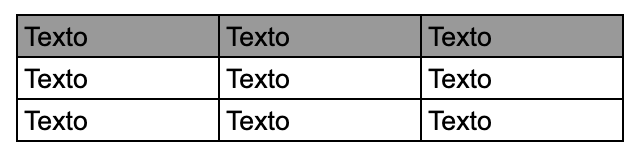
\includegraphics[height=3cm]{img/tablaejemplo.png}
%        \label{img:referencia3}
%    \end{measuredfigure}
%    \\ \textit{\scriptsize{Texto opcional al el pie de Tabla.}}
%\end{table}

\newpage
\subsection{Usar plantillas}
Pueden copiar y modificar el código que aparece a continuación en él .tex:

\begin{minipage}[H]{0.49\textwidth}
    \begin{table}[H]
        \centering
        \begin{measuredfigure}
            \caption{Tabla de referencia 2}
            \begin{tabular}{| l | c | r |}
            \hline
                \textbf{Texto} & \textbf{Texto} & \textbf{Texto} \\ \hline
                Textoblabla    & Textoblabla   & Textoblabla \\ \hline
                Texto    & Texto   & Texto \\ \hline
            \end{tabular}
        \end{measuredfigure}
    \end{table}
\end{minipage}
\begin{minipage}[H]{0.49\textwidth}
    \begin{table}[H]
        \centering
        \begin{measuredfigure}
            \caption{Tabla de referencia 3}
            \begin{tabular}{l l l}
            \toprule
                \textbf{Texto} & \textbf{Texto} & \textbf{Texto} \\
                \midrule
                Textoblabla    & Textoblabla   & Textoblabla \\
                Texto    & Texto   & Texto \\
                \bottomrule
            \end{tabular}
        \end{measuredfigure}
    \end{table}
\end{minipage}

\section{Fórmulas y Ecuaciones}

En LaTeX, puedes incluir fórmulas y ecuaciones matemáticas dentro del texto o en línea, como $E = mc^2$, utilizando el símbolo del dólar (\$) para abrir y cerrar la fórmula. Pueden buscar guías detalladas sobre como funcionan, sin embargo, con el correo universitario los estudiantes tienen acceso a \href{https://mathpix.com}{Mathpix} una aplicación móvil y de escritorio que digitaliza fórmulas en el formato deseado con muy buenos resultados.

También puedes crear ecuaciones numeradas como esta:

\begin{equation}
    a^2 + b^2 = c^2
\end{equation}

Puedes alinear varias ecuaciones utilizando el entorno \verb|\begin{align}|:

\begin{align}
    x &= 2y + 3 \\
    3x - 5y &= 9
\end{align}

Si no quieres numerar una ecuación, utiliza el entorno \verb|\begin{align*}|:

\begin{align*}
    f(x) &= x^2 + 2x + 1 \\
    &= (x + 1)^2
\end{align*}

%%%%%%%%%%%%%%%%%%%%%%%%%%%%%%%%%%%%%%%%%%%%%%%%%%%%%%%
\newpage
\section{TUTORIAL: Citación}

Tal como se indica en el archivo main, existen dos enfoques para agregar bibliografía en un documento \LaTeX. El primero implica la utilización de un archivo .bib, lo cual automatiza el proceso de citación. Al emplear esta técnica, se debe incluir el estilo de bibliografía mediante el comando \verb|\bibliographystyle{apacite}|, y luego referirse al archivo .bib con la instrucción \verb|\bibliography{mybib.bib}|, donde mybib.bib es el nombre del archivo de bibliografía. Este método es altamente automatizado y simplifica la tarea de referenciar.

La segunda opción implica agregar la bibliografía directamente en un archivo \textbf{.tex}, lo que resulta más manual. En este caso, se citan las fuentes manualmente utilizando comandos como \verb|\cite{key}| y se define el formato de la bibliografía utilizando \verb|\begin{thebibliography}{99}| y \verb|\end{thebibliography}|. Aunque menos automatizado que el primer enfoque, esta opción permite un mayor control sobre la presentación y organización de las referencias en el documento.

\subsection{Citas extensas}

Para citación extensa en formato APA, citas con más de 40 palabras, se sugiere el uso del siguiente comando personalizado:

\begin{verbatim}
    \quotex{cita}
    Ejemplo:
    \quotex{\lipsum (Autor, Año)}
\end{verbatim}

\quotex{...texto extenso... (Autor, Año)}

Puedes realizarlo de forma manual modificando el código comentado

%Cita extensa APA manual:

%\begin{flushright}
%    \begin{minipage}{0.96\linewidth}
%        \vspace{5pt}
%        {\small
%            %Acá va la cita
%        }
%        \vspace{5pt}
%    \end{minipage}
%\end{flushright}

\newpage  % BORRAR!
%%%%%%%%%%%%%%%%%%%%%%%% CONTENIDO %%%%%%%%%%%%%%%%%%%%%%%%%%%%%%%%
% Seleccionar uno de los siguientes apartados:
% TITULO
\begin{center}
    \LARGE
    \textbf{Título de la investigación experimental}
    \label{sec:investigacion_experimental}
    
    \vspace{0.4cm}
    \large
    Alumno $1^a$, (…) Profesor $1^b$ 

    \vspace{0.4cm}
\end{center}

% Informacion
\begin{enumerate}[label=\alph*]
    \item Indicar major o departamento, indicar escuela o
facultad, indicar universidad. Año de carrera, e-mail
    \item Indicar departamento, indicar escuela o facultad,
indicar universidad. Incluir categoría profesor, e-mail
\end{enumerate}

\hrulefill

\section*{Resumen}

El resumen debe indicar brevemente cuál es el problema, el objetivo o
hipótesis del estudio, métodos utilizados, resultados y conclusiones.
Además, debe ser independiente del texto principal, es decir, debe
entenderse por sí solo. \textbf{Extensión máxima: 300 palabras.}

\emph{\textbf{Palabras clave:}} incluir hasta 5 palabras claves que se
relacionen con el alcance y objetivo de la investigación.

\hrulefill

\textbf{NOTA: Si usted realizó una investigación de tipo
bibliográfica (recopilando información sin datos experimentales), ignore
esta plantilla y continúe \hyperref[sec:investigacion_bibliografica]{aquí}. De lo contrario, elimine esta instrucción.}

\section{Introducción}

Escriba aquí una breve introducción al tema de investigación, incluyendo
el estado del arte, su contingencia en Chile y/o en el mundo y el
desafío particular a resolver. La introducción debe: (1) indicar el
problema que justifica la investigación y/o la hipótesis en la que ésta
se basa, (2) los antecedentes o resultados de otros artículos que serán
utilizados durante el artículo, y (3) una explicación del enfoque
general y los objetivos del trabajo.

\subsection{Subsecciones}

Si necesita utilizar subsecciones para estructurar su escrito, puede
realizarlo siguiendo este formato. Esto es válido para las secciones
principales de este documento (Introducción, Metodología, Resultados y
Conclusión).

\section{Experimentación o metodología (según corresponda)}

En esta sección se describirá brevemente la metodología relevante en
relación al trabajo, indicando los experimentos o simulaciones
realizadas. De ser adecuado, incluya una descripción de los materiales
utilizados. La sección de metodología debe ser ordenada de manera lógica
(cronológicamente, por experimento, etc.) y puede incluir figuras,
tablas y/o referencias.

Algunas sugerencias de subsecciones son: Instrumentos, Grupos de estudio

\section{Resultados y discusión}

Describa y explique los principales resultados del trabajo presentado,
incluyendo un contraste con el estado del arte. Use tablas y figuras que
ayuden a una mejor comprensión de los resultados encontrados. Le
recordamos que la discusión debe incluir una interpretación de los
resultados obtenidos a la luz del problema o hipótesis planteados en la
introducción.

\section{Conclusiones}

Describa aquí las conclusiones del trabajo presentado. En ellas se deben
mencionar los resultados obtenidos más relevantes, las inferencias que
se extraen a partir de los resultados y las implicancias para el uso
práctico de ellas. Es importante destacar si
la hipótesis presentada fue refutada o no y cuál es el aporte de los
resultados al problema planteado.

\section*{Agradecimientos}

Puede incluir un reconocimiento a las personas o entidades que hayan
contribuido al estudio. Se debe especificar el tipo de apoyo entregado.

\section{Glosario}\label{glosario}

Debe incluir un máximo de 10 palabras o conceptos para
facilitar la lectura del público no especialista. La palabra a definir
debe aparecer en \textbf{NEGRITA} y mayúsculas la primera vez que se mencione en
el texto. Las palabras clave deben ser incluidas en el glosario y estar
listadas en orden alfabético. Evite anglicismos a menos que sea
estrictamente necesario.\\ Utilice el siguiente formato:


\begin{description}
    \definiritem{Palabra 1}{Definición de la palabra 1.}
    \definiritem{Palabra 2}{Definición de la palabra 2.}
    \definiritem{Palabra 3}{Definición de la palabra 3.}
\end{description}


\section*{Referencias}
El número de referencias es limitado a un máximo de 20 por artículo y
deberán seguir el estilo la \textbf{American Psychological Association
(APA).} Puede encontrar una guía detallada sobre su uso en el sitio web
de
\href{https://guiastematicas.bibliotecas.uc.cl/apa7}{Bibliotecas
UC}.


\newpage
\newpage
% TITULO
\begin{center}
    \LARGE
    \textbf{Investigación bibliográfica}
    \label{sec:investigacion_bibliografica}
    
    \vspace{0.4cm}
    \large
    Alumno $1^a$, (…) Profesor $1^b$ 

    \vspace{0.4cm}
\end{center}

% Informacion
\begin{enumerate}[label=\alph*]
    \item Indicar major o departamento, indicar escuela o
facultad, indicar universidad. Año de carrera, e-mail
    \item Indicar departamento, indicar escuela o facultad,
indicar universidad. Incluir categoría profesor, e-mail
\end{enumerate}

\hrulefill

\section*{Resumen}

El resumen debe indicar brevemente el estado del arte de la disciplina y la contribución de su recopilación. Esta sección debe ser independiente del texto principal, es decir, debe entenderse por sí misma. \textbf{Extensión máxima: 300 palabras.}

\textit{\textbf{Palabras clave:}} incluir hasta 5 palabras claves que se relacionen con el alcance y objetivo de la investigación.

\hrulefill


\section*{Cuerpo principal del texto}

Incluya aquí su investigación bibliográfica. Si bien su estructura es libre, se sugiere usar secciones y sub-secciones para facilitar su comprensión. Puede utilizar figuras o esquemas para guiar al lector. \textbf{El formato de preparación de referencias y material gráfico se mantienen.}

\textbf{La extensión máxima de texto y figuras es la misma que para los informes de investigación experimental}.

\emph{Una vez concluido su informe, elimine las secciones de ayuda previo al envío.}

\newpage
%%%%%%%%%%%%%%%%%%%%%%% FICHA DE INFORMACION %%%%%%%%%%%%%%%%%%%%%%
\fichaparteuno{Nombre completo}{Nombre mentor}
        {ejemplo@uc.cl}{ejemplo@uc.cl}
        {Sigla curso}{Seccion}
        {Año}{Semestre}
        {Titulo investigación}
\fichapartedos{Titulo del proyecto}
        {Fecha inicio}{\today}
        {}{X} % Escoger una
        {X}{} % Escoger una
        {NOMBRE MENTOR PRINCIPAL}{\today}

\end{lstlisting}

Por lo tanto, es importante considerar las siguientes indicaciones:
\begin{itemize}
    \item Al entregar el informe, se debe \textbf{eliminar} la sección de instrucciones y tutorial.
    \item En la parte de contenido, se debe seleccionar \textbf{únicamente 1} de los dos apartados disponibles.
    \item Se debe completar e imprimir la "Ficha de información" para que sea firmada y luego entregada en formato digital. \textbf{No} se tiene que incluir en el informe final. Una vez que esté firmada y en formato impreso, se debe eliminar dicha sección.
\end{itemize}


\section{TUTORIAL: Imágenes}

El contenido de la figura deberá estar en idioma inglés. La resolución de las imágenes debe ser de al menos 300 dpi y cada figura debe caber en una página tamaño carta (8,5 x 11 pulgadas). La revista utiliza tres tamaños estándar de figura: 1 columna, 85 mm; 1,5 columnas, 114 mm; y 2 columnas, 174 mm (ancho total de la página). Por favor, considere estas dimensiones al crear sus ilustraciones, aunque estas podrán ser encogidas durante el proceso de diseño editorial.

Los textos de las figuras deben ser en mayúsculas solo para la primera palabra de cada frase. Las unidades de medida deben tener un espacio entre el número y la unidad y seguir la nomenclatura internacional SI (por ejemplo, h en vez de hrs.). La numeración debe incluir “,” para separación de miles y “.” para separación de decimales.


\subsection{Imagen centrada}
En esta plantilla hay 2 formas de incluir imágenes. La primera es la más compleja y manual que aparece en el código comentado.
%\begin{figure}[H]
%    \centering
%    \begin{measuredfigure} % Lo usamos para aliniar el caption
%        
\includegraphics[width=0.2\textwidth]{img/cuadradoejemplo.png} % Alternativa \includegraphics[height=3cm]{}
%        \caption{Título de la imagen}
%        \label{img:label_referencia0}
%    \end{measuredfigure}
%\end{figure}

La segunda forma de incluir imágenes es la más sencilla, solo se tiene que usar el comando personalizado:
\begin{verbatim}
\fig[label]{Titulo}{tamaño}{ruta_imagen}
Ejemplo:
\fig[referencia1]{Titulo de la imagen 1}{width = 0.2\textwidth}{img/cuadradoejemplo.png}
\end{verbatim}

\fig[labelreferencia1]{Titulo de la imagen 1}{width = 0.2\textwidth}{img/cuadradoejemplo.png}


\subsection{Imágenes compuestas}

Para crear imágenes compuestas se requiere una mayor personalización, por lo que no se incluyo un comando para simplificarlo. Se pueden fijar en el código de este apartado.

\begin{figure}[H]
 \centering
  \subfloat[Foto1]{
    
\includegraphics[width=0.2\textwidth]{cuadradoejemplo.png}}
    \label{f:label_foto1}
  \subfloat[Foto2]{
    
\includegraphics[width=0.2\textwidth]{cuadradoejemplo.png}}
    \label{f:label_foto2}
  \subfloat[Foto3]{
    
\includegraphics[width=0.2\textwidth]{cuadradoejemplo.png}}
    \label{f:label_foto3}
 \caption{Múltiples imágenes}
 \label{f:label_multiples_imagenes}
\end{figure}

\subsection{Imágenes alineadas}
Si se desea incluir una imagen a la izquierda o derecha de un párrafo, se puede usar el siguiente comando (Poniendo \{r\} o \{l\} dependiendo del caso):
\begin{verbatim}
\figposition[label]{Titulo}{tamaño}{ruta_imagen}{posicion_r/l}
Ejemplo:
\figposition[referencia2]{Imagen referencia }{height=3cm}{img/cuadradoejemplo.png}{r}
\end{verbatim}

\figposition[referencia2]{Imagen referencia }{height=3cm}{img/cuadradoejemplo.png}{r}
% FORMA MANUAL:
%\begin{wrapfigure}{r}{0.25\textwidth} % Margen del texto
%    \centering
%    \begin{measuredfigure}
%        \caption{Imagen referencia 2}
%        
\includegraphics[height=3cm]{img/cuadradoejemplo.png} %[scale=0.1]
%        \label{img:referencia2}
%    \end{measuredfigure}
%\end{wrapfigure}
\textcolor{silver}{
    Lorem Ipsum is simply dummy text of the printing and typesetting industry. Lorem Ipsum has been the industry's standard dummy text ever since the 1500s, when an unknown printer took a galley of type and scrambled it to make a type specimen book. It has survived not only five centuries, but also the leap into electronic typesetting, remaining essentially unchanged.
    }

%%%%%%%%%%%%%%%%%%%%%%%%%%%%%%%%%%%%%%%%%%%%%%%%%%%%%%%
\newpage
\section{TUTORIAL: Tablas}

Se requiere utilizar "," para la unidad decimal, tanto en las tablas como en el texto.

Hacer tablas en \LaTeX es muy engorroso, por lo que presentamos 3 alternativas. Sin embargo, es necesario aclarar que para que se respete el formato de las tablas, \textbf{se tiene que poner el catión SOBRE la tabla.}

\subsection{Generador online}
Hay muchas páginas para generar tablas automáticamente, una alternativa es \href{https://www.tablesgenerator.com}{tablesgenerator}, sin embargo, este método genera muchas líneas innecesarias y cuando se incorporan párrafos muy grandes hay que ajustar las palabras.

\subsection{Insertar una imagen como tabla}
Se puede incorporar una imagen (De Excel, por ejemplo) como si fuera una tabla. El único inconveniente es que no va a permitir seleccionar el texto en el pdf generado. Al igual que con las imágenes, hay un comando personalizado y un código manual comentado.
\begin{verbatim}
\tableimage[label]{Titulo}{tamaño}{ruta_imagen}
Ejemplo:
\tableimage[referencia3]{Tabla de referencia 1}{height=3cm}{img/tablaejemplo.png}
\end{verbatim}



\tableimage[referencia3]{Titulo de la tabla de referencia}{height=3cm}{img/tablaejemplo.png}

% Tabla manual:
%\begin{table}[H]
%    \centering
%    \begin{measuredfigure}
%        \caption{Tabla de referencia 1}
%        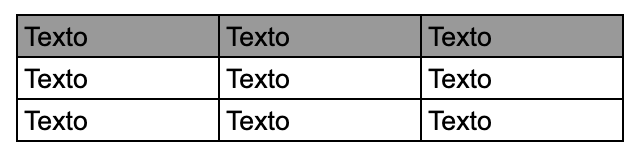
\includegraphics[height=3cm]{img/tablaejemplo.png}
%        \label{img:referencia3}
%    \end{measuredfigure}
%    \\ \textit{\scriptsize{Texto opcional al el pie de Tabla.}}
%\end{table}

\newpage
\subsection{Usar plantillas}
Pueden copiar y modificar el código que aparece a continuación en él .tex:

\begin{minipage}[H]{0.49\textwidth}
    \begin{table}[H]
        \centering
        \begin{measuredfigure}
            \caption{Tabla de referencia 2}
            \begin{tabular}{| l | c | r |}
            \hline
                \textbf{Texto} & \textbf{Texto} & \textbf{Texto} \\ \hline
                Textoblabla    & Textoblabla   & Textoblabla \\ \hline
                Texto    & Texto   & Texto \\ \hline
            \end{tabular}
        \end{measuredfigure}
    \end{table}
\end{minipage}
\begin{minipage}[H]{0.49\textwidth}
    \begin{table}[H]
        \centering
        \begin{measuredfigure}
            \caption{Tabla de referencia 3}
            \begin{tabular}{l l l}
            \toprule
                \textbf{Texto} & \textbf{Texto} & \textbf{Texto} \\
                \midrule
                Textoblabla    & Textoblabla   & Textoblabla \\
                Texto    & Texto   & Texto \\
                \bottomrule
            \end{tabular}
        \end{measuredfigure}
    \end{table}
\end{minipage}

\section{Fórmulas y Ecuaciones}

En LaTeX, puedes incluir fórmulas y ecuaciones matemáticas dentro del texto o en línea, como $E = mc^2$, utilizando el símbolo del dólar (\$) para abrir y cerrar la fórmula. Pueden buscar guías detalladas sobre como funcionan, sin embargo, con el correo universitario los estudiantes tienen acceso a \href{https://mathpix.com}{Mathpix} una aplicación móvil y de escritorio que digitaliza fórmulas en el formato deseado con muy buenos resultados.

También puedes crear ecuaciones numeradas como esta:

\begin{equation}
    a^2 + b^2 = c^2
\end{equation}

Puedes alinear varias ecuaciones utilizando el entorno \verb|\begin{align}|:

\begin{align}
    x &= 2y + 3 \\
    3x - 5y &= 9
\end{align}

Si no quieres numerar una ecuación, utiliza el entorno \verb|\begin{align*}|:

\begin{align*}
    f(x) &= x^2 + 2x + 1 \\
    &= (x + 1)^2
\end{align*}

%%%%%%%%%%%%%%%%%%%%%%%%%%%%%%%%%%%%%%%%%%%%%%%%%%%%%%%
\newpage
\section{TUTORIAL: Citación}

Tal como se indica en el archivo main, existen dos enfoques para agregar bibliografía en un documento \LaTeX. El primero implica la utilización de un archivo .bib, lo cual automatiza el proceso de citación. Al emplear esta técnica, se debe incluir el estilo de bibliografía mediante el comando \verb|\bibliographystyle{apacite}|, y luego referirse al archivo .bib con la instrucción \verb|\bibliography{mybib.bib}|, donde mybib.bib es el nombre del archivo de bibliografía. Este método es altamente automatizado y simplifica la tarea de referenciar.

La segunda opción implica agregar la bibliografía directamente en un archivo \textbf{.tex}, lo que resulta más manual. En este caso, se citan las fuentes manualmente utilizando comandos como \verb|\cite{key}| y se define el formato de la bibliografía utilizando \verb|\begin{thebibliography}{99}| y \verb|\end{thebibliography}|. Aunque menos automatizado que el primer enfoque, esta opción permite un mayor control sobre la presentación y organización de las referencias en el documento.

\subsection{Citas extensas}

Para citación extensa en formato APA, citas con más de 40 palabras, se sugiere el uso del siguiente comando personalizado:

\begin{verbatim}
    \quotex{cita}
    Ejemplo:
    \quotex{\lipsum (Autor, Año)}
\end{verbatim}

\quotex{...texto extenso... (Autor, Año)}

Puedes realizarlo de forma manual modificando el código comentado

%Cita extensa APA manual:

%\begin{flushright}
%    \begin{minipage}{0.96\linewidth}
%        \vspace{5pt}
%        {\small
%            %Acá va la cita
%        }
%        \vspace{5pt}
%    \end{minipage}
%\end{flushright}

\newpage  % BORRAR!
%%%%%%%%%%%%%%%%%%%%%%%% CONTENIDO %%%%%%%%%%%%%%%%%%%%%%%%%%%%%%%%
% Seleccionar uno de los siguientes apartados:
% TITULO
\begin{center}
    \LARGE
    \textbf{Título de la investigación experimental}
    \label{sec:investigacion_experimental}
    
    \vspace{0.4cm}
    \large
    Alumno $1^a$, (…) Profesor $1^b$ 

    \vspace{0.4cm}
\end{center}

% Informacion
\begin{enumerate}[label=\alph*]
    \item Indicar major o departamento, indicar escuela o
facultad, indicar universidad. Año de carrera, e-mail
    \item Indicar departamento, indicar escuela o facultad,
indicar universidad. Incluir categoría profesor, e-mail
\end{enumerate}

\hrulefill

\section*{Resumen}

El resumen debe indicar brevemente cuál es el problema, el objetivo o
hipótesis del estudio, métodos utilizados, resultados y conclusiones.
Además, debe ser independiente del texto principal, es decir, debe
entenderse por sí solo. \textbf{Extensión máxima: 300 palabras.}

\emph{\textbf{Palabras clave:}} incluir hasta 5 palabras claves que se
relacionen con el alcance y objetivo de la investigación.

\hrulefill

\textbf{NOTA: Si usted realizó una investigación de tipo
bibliográfica (recopilando información sin datos experimentales), ignore
esta plantilla y continúe \hyperref[sec:investigacion_bibliografica]{aquí}. De lo contrario, elimine esta instrucción.}

\section{Introducción}

Escriba aquí una breve introducción al tema de investigación, incluyendo
el estado del arte, su contingencia en Chile y/o en el mundo y el
desafío particular a resolver. La introducción debe: (1) indicar el
problema que justifica la investigación y/o la hipótesis en la que ésta
se basa, (2) los antecedentes o resultados de otros artículos que serán
utilizados durante el artículo, y (3) una explicación del enfoque
general y los objetivos del trabajo.

\subsection{Subsecciones}

Si necesita utilizar subsecciones para estructurar su escrito, puede
realizarlo siguiendo este formato. Esto es válido para las secciones
principales de este documento (Introducción, Metodología, Resultados y
Conclusión).

\section{Experimentación o metodología (según corresponda)}

En esta sección se describirá brevemente la metodología relevante en
relación al trabajo, indicando los experimentos o simulaciones
realizadas. De ser adecuado, incluya una descripción de los materiales
utilizados. La sección de metodología debe ser ordenada de manera lógica
(cronológicamente, por experimento, etc.) y puede incluir figuras,
tablas y/o referencias.

Algunas sugerencias de subsecciones son: Instrumentos, Grupos de estudio

\section{Resultados y discusión}

Describa y explique los principales resultados del trabajo presentado,
incluyendo un contraste con el estado del arte. Use tablas y figuras que
ayuden a una mejor comprensión de los resultados encontrados. Le
recordamos que la discusión debe incluir una interpretación de los
resultados obtenidos a la luz del problema o hipótesis planteados en la
introducción.

\section{Conclusiones}

Describa aquí las conclusiones del trabajo presentado. En ellas se deben
mencionar los resultados obtenidos más relevantes, las inferencias que
se extraen a partir de los resultados y las implicancias para el uso
práctico de ellas. Es importante destacar si
la hipótesis presentada fue refutada o no y cuál es el aporte de los
resultados al problema planteado.

\section*{Agradecimientos}

Puede incluir un reconocimiento a las personas o entidades que hayan
contribuido al estudio. Se debe especificar el tipo de apoyo entregado.

\section{Glosario}\label{glosario}

Debe incluir un máximo de 10 palabras o conceptos para
facilitar la lectura del público no especialista. La palabra a definir
debe aparecer en \textbf{NEGRITA} y mayúsculas la primera vez que se mencione en
el texto. Las palabras clave deben ser incluidas en el glosario y estar
listadas en orden alfabético. Evite anglicismos a menos que sea
estrictamente necesario.\\ Utilice el siguiente formato:


\begin{description}
    \definiritem{Palabra 1}{Definición de la palabra 1.}
    \definiritem{Palabra 2}{Definición de la palabra 2.}
    \definiritem{Palabra 3}{Definición de la palabra 3.}
\end{description}


\section*{Referencias}
El número de referencias es limitado a un máximo de 20 por artículo y
deberán seguir el estilo la \textbf{American Psychological Association
(APA).} Puede encontrar una guía detallada sobre su uso en el sitio web
de
\href{https://guiastematicas.bibliotecas.uc.cl/apa7}{Bibliotecas
UC}.


\newpage
\newpage
% TITULO
\begin{center}
    \LARGE
    \textbf{Investigación bibliográfica}
    \label{sec:investigacion_bibliografica}
    
    \vspace{0.4cm}
    \large
    Alumno $1^a$, (…) Profesor $1^b$ 

    \vspace{0.4cm}
\end{center}

% Informacion
\begin{enumerate}[label=\alph*]
    \item Indicar major o departamento, indicar escuela o
facultad, indicar universidad. Año de carrera, e-mail
    \item Indicar departamento, indicar escuela o facultad,
indicar universidad. Incluir categoría profesor, e-mail
\end{enumerate}

\hrulefill

\section*{Resumen}

El resumen debe indicar brevemente el estado del arte de la disciplina y la contribución de su recopilación. Esta sección debe ser independiente del texto principal, es decir, debe entenderse por sí misma. \textbf{Extensión máxima: 300 palabras.}

\textit{\textbf{Palabras clave:}} incluir hasta 5 palabras claves que se relacionen con el alcance y objetivo de la investigación.

\hrulefill


\section*{Cuerpo principal del texto}

Incluya aquí su investigación bibliográfica. Si bien su estructura es libre, se sugiere usar secciones y sub-secciones para facilitar su comprensión. Puede utilizar figuras o esquemas para guiar al lector. \textbf{El formato de preparación de referencias y material gráfico se mantienen.}

\textbf{La extensión máxima de texto y figuras es la misma que para los informes de investigación experimental}.

\emph{Una vez concluido su informe, elimine las secciones de ayuda previo al envío.}

\newpage
%%%%%%%%%%%%%%%%%%%%%%% FICHA DE INFORMACION %%%%%%%%%%%%%%%%%%%%%%
\fichaparteuno{Nombre completo}{Nombre mentor}
        {ejemplo@uc.cl}{ejemplo@uc.cl}
        {Sigla curso}{Seccion}
        {Año}{Semestre}
        {Titulo investigación}
\fichapartedos{Titulo del proyecto}
        {Fecha inicio}{\today}
        {}{X} % Escoger una
        {X}{} % Escoger una
        {NOMBRE MENTOR PRINCIPAL}{\today}

\end{lstlisting}

Por lo tanto, es importante considerar las siguientes indicaciones:
\begin{itemize}
    \item Al entregar el informe, se debe \textbf{eliminar} la sección de instrucciones y tutorial.
    \item En la parte de contenido, se debe seleccionar \textbf{únicamente 1} de los dos apartados disponibles.
    \item Se debe completar e imprimir la "Ficha de información" para que sea firmada y luego entregada en formato digital. \textbf{No} se tiene que incluir en el informe final. Una vez que esté firmada y en formato impreso, se debe eliminar dicha sección.
\end{itemize}


\section{TUTORIAL: Imágenes}

El contenido de la figura deberá estar en idioma inglés. La resolución de las imágenes debe ser de al menos 300 dpi y cada figura debe caber en una página tamaño carta (8,5 x 11 pulgadas). La revista utiliza tres tamaños estándar de figura: 1 columna, 85 mm; 1,5 columnas, 114 mm; y 2 columnas, 174 mm (ancho total de la página). Por favor, considere estas dimensiones al crear sus ilustraciones, aunque estas podrán ser encogidas durante el proceso de diseño editorial.

Los textos de las figuras deben ser en mayúsculas solo para la primera palabra de cada frase. Las unidades de medida deben tener un espacio entre el número y la unidad y seguir la nomenclatura internacional SI (por ejemplo, h en vez de hrs.). La numeración debe incluir “,” para separación de miles y “.” para separación de decimales.


\subsection{Imagen centrada}
En esta plantilla hay 2 formas de incluir imágenes. La primera es la más compleja y manual que aparece en el código comentado.
%\begin{figure}[H]
%    \centering
%    \begin{measuredfigure} % Lo usamos para aliniar el caption
%        
\includegraphics[width=0.2\textwidth]{img/cuadradoejemplo.png} % Alternativa \includegraphics[height=3cm]{}
%        \caption{Título de la imagen}
%        \label{img:label_referencia0}
%    \end{measuredfigure}
%\end{figure}

La segunda forma de incluir imágenes es la más sencilla, solo se tiene que usar el comando personalizado:
\begin{verbatim}
\fig[label]{Titulo}{tamaño}{ruta_imagen}
Ejemplo:
\fig[referencia1]{Titulo de la imagen 1}{width = 0.2\textwidth}{img/cuadradoejemplo.png}
\end{verbatim}

\fig[labelreferencia1]{Titulo de la imagen 1}{width = 0.2\textwidth}{img/cuadradoejemplo.png}


\subsection{Imágenes compuestas}

Para crear imágenes compuestas se requiere una mayor personalización, por lo que no se incluyo un comando para simplificarlo. Se pueden fijar en el código de este apartado.

\begin{figure}[H]
 \centering
  \subfloat[Foto1]{
    
\includegraphics[width=0.2\textwidth]{cuadradoejemplo.png}}
    \label{f:label_foto1}
  \subfloat[Foto2]{
    
\includegraphics[width=0.2\textwidth]{cuadradoejemplo.png}}
    \label{f:label_foto2}
  \subfloat[Foto3]{
    
\includegraphics[width=0.2\textwidth]{cuadradoejemplo.png}}
    \label{f:label_foto3}
 \caption{Múltiples imágenes}
 \label{f:label_multiples_imagenes}
\end{figure}

\subsection{Imágenes alineadas}
Si se desea incluir una imagen a la izquierda o derecha de un párrafo, se puede usar el siguiente comando (Poniendo \{r\} o \{l\} dependiendo del caso):
\begin{verbatim}
\figposition[label]{Titulo}{tamaño}{ruta_imagen}{posicion_r/l}
Ejemplo:
\figposition[referencia2]{Imagen referencia }{height=3cm}{img/cuadradoejemplo.png}{r}
\end{verbatim}

\figposition[referencia2]{Imagen referencia }{height=3cm}{img/cuadradoejemplo.png}{r}
% FORMA MANUAL:
%\begin{wrapfigure}{r}{0.25\textwidth} % Margen del texto
%    \centering
%    \begin{measuredfigure}
%        \caption{Imagen referencia 2}
%        
\includegraphics[height=3cm]{img/cuadradoejemplo.png} %[scale=0.1]
%        \label{img:referencia2}
%    \end{measuredfigure}
%\end{wrapfigure}
\textcolor{silver}{
    Lorem Ipsum is simply dummy text of the printing and typesetting industry. Lorem Ipsum has been the industry's standard dummy text ever since the 1500s, when an unknown printer took a galley of type and scrambled it to make a type specimen book. It has survived not only five centuries, but also the leap into electronic typesetting, remaining essentially unchanged.
    }

%%%%%%%%%%%%%%%%%%%%%%%%%%%%%%%%%%%%%%%%%%%%%%%%%%%%%%%
\newpage
\section{TUTORIAL: Tablas}

Se requiere utilizar "," para la unidad decimal, tanto en las tablas como en el texto.

Hacer tablas en \LaTeX es muy engorroso, por lo que presentamos 3 alternativas. Sin embargo, es necesario aclarar que para que se respete el formato de las tablas, \textbf{se tiene que poner el catión SOBRE la tabla.}

\subsection{Generador online}
Hay muchas páginas para generar tablas automáticamente, una alternativa es \href{https://www.tablesgenerator.com}{tablesgenerator}, sin embargo, este método genera muchas líneas innecesarias y cuando se incorporan párrafos muy grandes hay que ajustar las palabras.

\subsection{Insertar una imagen como tabla}
Se puede incorporar una imagen (De Excel, por ejemplo) como si fuera una tabla. El único inconveniente es que no va a permitir seleccionar el texto en el pdf generado. Al igual que con las imágenes, hay un comando personalizado y un código manual comentado.
\begin{verbatim}
\tableimage[label]{Titulo}{tamaño}{ruta_imagen}
Ejemplo:
\tableimage[referencia3]{Tabla de referencia 1}{height=3cm}{img/tablaejemplo.png}
\end{verbatim}



\tableimage[referencia3]{Titulo de la tabla de referencia}{height=3cm}{img/tablaejemplo.png}

% Tabla manual:
%\begin{table}[H]
%    \centering
%    \begin{measuredfigure}
%        \caption{Tabla de referencia 1}
%        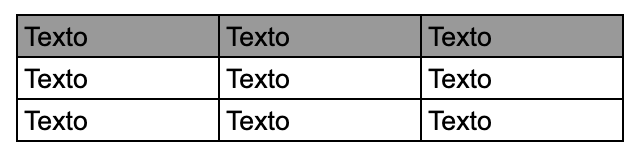
\includegraphics[height=3cm]{img/tablaejemplo.png}
%        \label{img:referencia3}
%    \end{measuredfigure}
%    \\ \textit{\scriptsize{Texto opcional al el pie de Tabla.}}
%\end{table}

\newpage
\subsection{Usar plantillas}
Pueden copiar y modificar el código que aparece a continuación en él .tex:

\begin{minipage}[H]{0.49\textwidth}
    \begin{table}[H]
        \centering
        \begin{measuredfigure}
            \caption{Tabla de referencia 2}
            \begin{tabular}{| l | c | r |}
            \hline
                \textbf{Texto} & \textbf{Texto} & \textbf{Texto} \\ \hline
                Textoblabla    & Textoblabla   & Textoblabla \\ \hline
                Texto    & Texto   & Texto \\ \hline
            \end{tabular}
        \end{measuredfigure}
    \end{table}
\end{minipage}
\begin{minipage}[H]{0.49\textwidth}
    \begin{table}[H]
        \centering
        \begin{measuredfigure}
            \caption{Tabla de referencia 3}
            \begin{tabular}{l l l}
            \toprule
                \textbf{Texto} & \textbf{Texto} & \textbf{Texto} \\
                \midrule
                Textoblabla    & Textoblabla   & Textoblabla \\
                Texto    & Texto   & Texto \\
                \bottomrule
            \end{tabular}
        \end{measuredfigure}
    \end{table}
\end{minipage}

\section{Fórmulas y Ecuaciones}

En LaTeX, puedes incluir fórmulas y ecuaciones matemáticas dentro del texto o en línea, como $E = mc^2$, utilizando el símbolo del dólar (\$) para abrir y cerrar la fórmula. Pueden buscar guías detalladas sobre como funcionan, sin embargo, con el correo universitario los estudiantes tienen acceso a \href{https://mathpix.com}{Mathpix} una aplicación móvil y de escritorio que digitaliza fórmulas en el formato deseado con muy buenos resultados.

También puedes crear ecuaciones numeradas como esta:

\begin{equation}
    a^2 + b^2 = c^2
\end{equation}

Puedes alinear varias ecuaciones utilizando el entorno \verb|\begin{align}|:

\begin{align}
    x &= 2y + 3 \\
    3x - 5y &= 9
\end{align}

Si no quieres numerar una ecuación, utiliza el entorno \verb|\begin{align*}|:

\begin{align*}
    f(x) &= x^2 + 2x + 1 \\
    &= (x + 1)^2
\end{align*}

%%%%%%%%%%%%%%%%%%%%%%%%%%%%%%%%%%%%%%%%%%%%%%%%%%%%%%%
\newpage
\section{TUTORIAL: Citación}

Tal como se indica en el archivo main, existen dos enfoques para agregar bibliografía en un documento \LaTeX. El primero implica la utilización de un archivo .bib, lo cual automatiza el proceso de citación. Al emplear esta técnica, se debe incluir el estilo de bibliografía mediante el comando \verb|\bibliographystyle{apacite}|, y luego referirse al archivo .bib con la instrucción \verb|\bibliography{mybib.bib}|, donde mybib.bib es el nombre del archivo de bibliografía. Este método es altamente automatizado y simplifica la tarea de referenciar.

La segunda opción implica agregar la bibliografía directamente en un archivo \textbf{.tex}, lo que resulta más manual. En este caso, se citan las fuentes manualmente utilizando comandos como \verb|\cite{key}| y se define el formato de la bibliografía utilizando \verb|\begin{thebibliography}{99}| y \verb|\end{thebibliography}|. Aunque menos automatizado que el primer enfoque, esta opción permite un mayor control sobre la presentación y organización de las referencias en el documento.

\subsection{Citas extensas}

Para citación extensa en formato APA, citas con más de 40 palabras, se sugiere el uso del siguiente comando personalizado:

\begin{verbatim}
    \quotex{cita}
    Ejemplo:
    \quotex{\lipsum (Autor, Año)}
\end{verbatim}

\quotex{...texto extenso... (Autor, Año)}

Puedes realizarlo de forma manual modificando el código comentado

%Cita extensa APA manual:

%\begin{flushright}
%    \begin{minipage}{0.96\linewidth}
%        \vspace{5pt}
%        {\small
%            %Acá va la cita
%        }
%        \vspace{5pt}
%    \end{minipage}
%\end{flushright}

\newpage